%% SOICT 2026 submission -- Springer CCIS / LNCS (llncs.cls).
%% 12 pages excluding references; single blind (authors shown); no page numbers.
%% CAMERA-READY: delete the two \pagestyle/\thispagestyle{empty} lines.

\documentclass[runningheads,a4paper]{llncs}

\usepackage[T5,T1]{fontenc}% T5: Vietnamese glyphs for the prompt in Appendix A
\usepackage[utf8]{inputenc}
\usepackage{amsmath}
\usepackage{amssymb}
\usepackage{booktabs}
\usepackage{array}
\usepackage{graphicx}
\usepackage{tikz}
\usepackage{marvosym}
\usepackage[hidelinks]{hyperref}

\setlength{\emergencystretch}{1.5em}
\newcommand{\vn}[1]{{\fontencoding{T5}\selectfont #1}}

\begin{document}

\title{GUIStep: A Compact Vision-Language Model\\
for GUI Step Instruction Generation}

\titlerunning{GUIStep}

\author{Uyen Le Doan Phuong\inst{1}\textsuperscript{(\Letter)}}

\authorrunning{U. Le Doan Phuong}

\institute{Faculty of Information Technology, University of Science, VNU-HCM,\\
Ho Chi Minh City, Vietnam\\
\email{24C15039@student.hcmus.edu.vn}}

\maketitle

\begin{abstract}
Most GUI agents map a screenshot and a goal to an action coordinate. We study the complementary
task of writing one sentence that tells a person which element to touch next, and present GUIStep, a
training framework that collects no new annotations. GUIStep reuses the human step
instructions in AndroidControl and derives from the accessibility tree a structured
\emph{declaration} of each target element (its role, name, position and a nearby landmark), giving
$64{,}567$ training examples. We adapt the compact Qwen2.5-VL-3B-Instruct with QLoRA in two ways, on
the sentence alone and on a declaration followed by the sentence, and refine the second model with
preference pairs that differ only in the declared element. Because one element can be described in
many valid ways, we score a sentence by execution: a frozen grounding model reads it and points to
the screen, and the step counts as correct when the point falls inside the intended element and the
action class matches. We call the share of correct steps \emph{executability}. On $4{,}463$
held-out touch steps, the preference-refined model reaches an executability of $66.5$, against
$53.6$ for the untuned backbone, and raises BLEU-4 from $15.3$ to $49.9$. Most of this gain,
however, comes from training on the sentence alone. Adding the declaration lowers executability by
$1.9$ points, and preference refinement recovers the loss without significantly exceeding the
sentence-only model. The ranking of all systems is unchanged under a stricter localisation rule and
with a listener from another model family.
\keywords{GUI instruction generation \and vision-language models \and mobile applications
\and user assistance \and evaluation metric}
\end{abstract}

%------------------------------------------------------------------------------
\section{Introduction}
\label{sec:intro}

A user who gets stuck halfway through a phone task needs to be told, in one sentence, what to touch next, for example \emph{Click on the share icon at the top right of the screen}. Sentences of this kind make up help pages and step-by-step user guides. Research on GUI agents mostly targets a different output. Agents such as SeeClick~\cite{seeclick} and OS-Atlas~\cite{osatlas}, and grounding models such as UGround~\cite{uground}, produce a machine-readable action such as \texttt{click(872,141)} so that software can act on the user's behalf, and any language they produce along the way is an intermediate step that is not evaluated. We instead generate the instruction itself, for a human reader (Fig.~\ref{fig:overview}).

\begin{figure}[!ht]
\centering
\begin{tikzpicture}[font=\footnotesize]
% screenshot node spans x in [0,3.3], y in [-3.373,0]; touch at 14.2% width, 33.2% height
\node[anchor=south west,text width=11.7cm,align=left,inner sep=0pt] at (0,0.2)
  {\textbf{Goal.} I travel with Aer Lingus Airlines regularly and like their service, so look up
  the flight details in the booking.com app and sort by the cheapest direct flight\\[2pt]
  \textbf{Previous steps.} Click on the airlines option at the top of the screen $\rightarrow$
  Click on Aer Lingus option $\rightarrow$ Click on done option};
\node[inner sep=0pt,anchor=north west] (img) at (0,0)
  {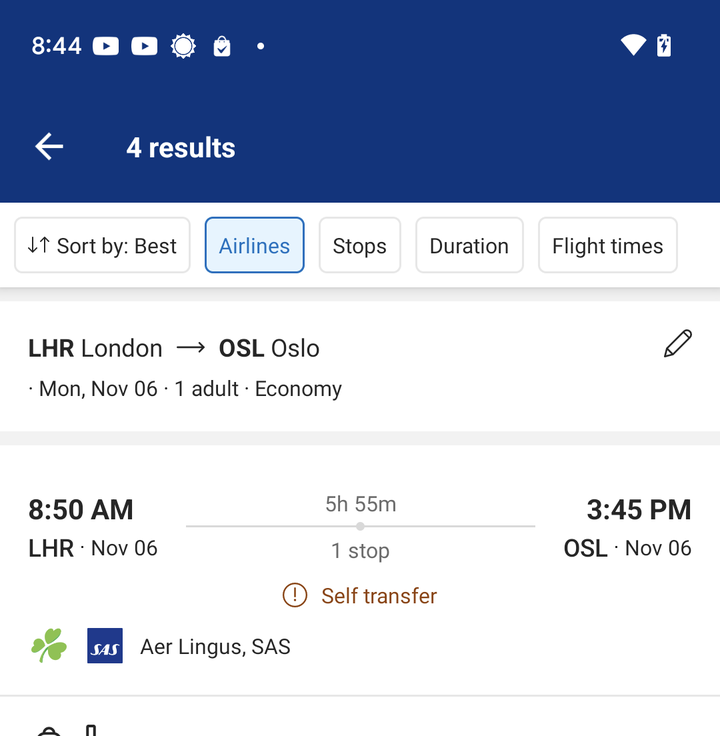
\includegraphics[width=3.3cm]{fig1_screen.png}};
\draw[red!70!black,line width=0.6pt] (0.468,-1.121) circle (2.9mm);
\fill[red!70!black] (0.468,-1.121) circle (0.3mm);
\node[draw,rounded corners,fill=black!6,anchor=west,align=center,
      minimum width=2cm,minimum height=0.9cm] (mod) at (3.9,-1.687)
  {GUIStep\\[-1pt]{\scriptsize (Sect.~\ref{sec:framework})}};
\node[anchor=west,text width=5.2cm,align=left] (out) at (6.5,-1.687)
  {\textbf{generated:} \emph{``Click on the sort by option''}};
\node[anchor=north west,text width=5.2cm,align=left] at (6.48,-2.0)
  {\textbf{reference:} \emph{``Click on sort by option at the top left of the screen''}};
\draw[->,thick] (3.45,-1.687) -- (3.85,-1.687);
\draw[->,thick] (5.95,-1.687) -- (6.4,-1.687);
\end{tikzpicture}
\caption{One step of the task, taken from an episode in the training split of
AndroidControl~\cite{androidcontrol} to illustrate the input and output. \mbox{GUIStep-P} saw this step
during training, so it is not a scored example. The OCR strings the model also reads are omitted.
Five filter chips compete on this screen, so the instruction has to name the intended one. The
circle marks the recorded touch and is not shown to the model.}
\label{fig:overview}
\end{figure}

GUIStep is a training framework that builds all of its supervision from what a recorded
demonstration already contains: the human instruction, the touched point and the UI structure tree.
We instantiate it on AndroidControl~\cite{androidcontrol} with Qwen2.5-VL-3B-Instruct~\cite{qwen25vl} in three configurations. \mbox{GUIStep-S} predicts the instruction directly. \mbox{GUIStep-D} first writes a structured declaration of the target element, so that the model commits to one element before describing it. \mbox{GUIStep-P} refines \mbox{GUIStep-D} with preference pairs that share an instruction but declare different elements. 

Scoring these sentences is hard, because the same button has many valid names and a single reference covers only one of them. \emph{Click on the search bar} and \emph{Tap the magnifying glass at the top} denote
one element, and no corpus lists the admissible wordings. In a small pilot with valid rewordings that we wrote, string matching on content words rejects $97.5\%$ of them. Similarity between sentence embeddings does no
better: on $51$ hand-written cases it separates rewordings of the same element from descriptions of
different elements with an AUC of $0.336$, below the $0.5$ of chance. It rewards a shared topic, so \texttt{inbox}/\texttt{outbox} reaches a cosine similarity of $0.76$, whereas \texttt{search}/\texttt{magnifying glass}, two names for one button, reaches $0.55$.

We therefore adopt the criterion used in referring expression generation, where a description is
adequate if a \emph{listener} recovers the referent~\cite{mao2016,luo2017,yu2016}. On phone screens our listener is a frozen grounding model that reads the sentence and returns a point. We call the share of steps on which this point falls on the intended element, with the right action named, \emph{executability}.  Because the listener is itself a learned model, we validate it before use. Reference instructions reach $83.8$ under this score, and we read all
results against that measured ceiling instead of against $100$.

Our main contributions are as follows.
\begin{itemize}
\item \textbf{GUIStep, a training framework for GUI step instruction generation} that derives
sentence targets, target declarations and preference pairs from recorded demonstrations without
collecting additional labels, instantiated on AndroidControl (Sects.~\ref{sec:framework}
and~\ref{sec:setup}).
\item \textbf{An execution-based score for the generated instructions.} We measure its ceiling and floor and its reaction to paraphrase, and show that the ranking of systems holds under a stricter rule and with a second listener from another model family (Sect.~\ref{sec:metric}).
\item \textbf{A controlled ablation.} With a matched cross-entropy control and a
select-then-verbalise variant, we show that most of the gain comes from training on the sentence,
while the declaration and the preference objective add no clear benefit beyond it
(Sect.~\ref{sec:results}).
\end{itemize}

%------------------------------------------------------------------------------
\section{Related Work}
\label{sec:related}

\paragraph{Language about graphical interfaces.}
Widget Captioning~\cite{widgetcap} writes a label for a UI element that has already been selected
and reports visually identical widgets as its hardest case. Screen2Words~\cite{screen2words}
summarises a whole screen, VUT~\cite{vut} shares one encoder across five UI tasks, and Spotlight~\cite{spotlight} and Ferret-UI~\cite{ferretui} describe a given region or locate the element that a given expression names. None of these systems decides which element should be acted on next. In our task the model has to make that decision before it can describe the element.

\paragraph{GUI control and grounding.}
AndroidControl~\cite{androidcontrol} records $15{,}283$ human episodes and uses each step's
instruction as \emph{input} to action prediction. We use the same instruction as the generation
target, and take our localisation rule from its Appendix~D.3. Android-in-the-Wild~\cite{aitw}
introduced the $0.14$ normalised tolerance that is widely used to judge a predicted coordinate;
Sect.~\ref{sec:rules} compares it with two other rules. Grounding
models~\cite{seeclick,osatlas,uground} map a referring expression to a point on the screen. We use
one as the \emph{listener} of our metric, not as a system under test, and Sect.~\ref{sec:validate}
reports its measured error and whether its training data include AndroidControl.

\paragraph{Listener-based evaluation.}
In referring expression generation, Mao et al.~\cite{mao2016} train a speaker so that its description singles out the target among the other objects, Luo and Shakhnarovich~\cite{luo2017} let the comprehension model
guide generation, and Yu et al.~\cite{yu2016} add the visual context of competing objects. Newman et
al.~\cite{newman2020} argue that a model listener tracks communicative success better than $n$-gram
overlap, and Zhao et al.~\cite{zhao2021} find that BLEU, ROUGE, METEOR and CIDEr fail to judge
navigation instructions; like us, they report a human reference beside the system scores. Our
injection suite follows the perturbation checklists of Sai et al.~\cite{sai2021}, which test whether
a metric reacts to controlled changes in the output. Clark et al.~\cite{clark2021} show that untrained
human judges cannot reliably tell generated text from human text, so human ratings are not a safe gold standard either. Jandial et al.~\cite{groundersunderstand} show that GUI grounders can be
misled by rephrased descriptions. Section~\ref{sec:validate} measures how our listener reacts to
paraphrases and to errors of known type.

%------------------------------------------------------------------------------
\section{The GUIStep Framework}
\label{sec:framework}

GUIStep consists of a task definition, a recipe for building supervision from records that a GUI dataset already contains, and an execution-based score. None of the three is specific to AndroidControl. The score needs only the screenshot, the sentence and the recorded touch, so it applies to any dataset that records touches. Figure~\ref{fig:pipeline} shows how they connect. Section~\ref{sec:metric} defines and validates the score, and Sect.~\ref{sec:setup} instantiates the framework on AndroidControl.

\begin{figure}[t]
\centering
\resizebox{\textwidth}{!}{%
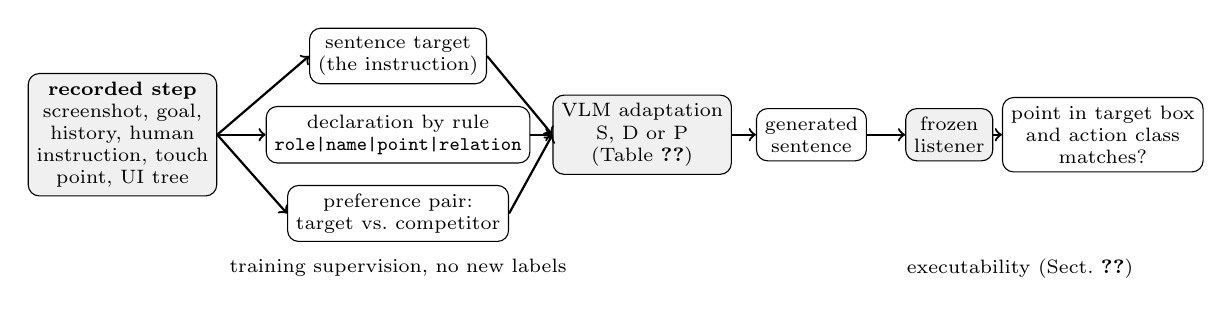
\begin{tikzpicture}[font=\scriptsize,
  box/.style={draw,rounded corners,align=center,inner sep=3pt},
  arr/.style={->,thick}]
\node[box,fill=black!6] (rec) at (0,0)
  {\textbf{recorded step}\\ screenshot, goal,\\ history, human\\ instruction, touch\\ point, UI tree};
\node[box] (sent) at (3.5,1.0) {sentence target\\ (the instruction)};
\node[box] (decl) at (3.5,0) {declaration by rule\\ \texttt{role|name|point|relation}};
\node[box] (pair) at (3.5,-1.0) {preference pair:\\ target vs.\ competitor};
\node[box,fill=black!6] (vlm) at (6.6,0) {VLM adaptation\\ S, D or P\\ (Table~\ref{tab:configs})};
\node[box] (out) at (8.75,0) {generated\\ sentence};
\node[box,fill=black!6] (lis) at (10.5,0) {frozen\\ listener};
\node[box] (sc) at (12.45,0) {point in target box\\ and action class\\ matches?};
\foreach \n in {sent,decl,pair} {\draw[arr] (rec.east) -- (\n.west); \draw[arr] (\n.east) -- (vlm.west);}
\draw[arr] (vlm) -- (out);
\draw[arr] (out) -- (lis);
\draw[arr] (lis) -- (sc);
\node[anchor=north] at (3.5,-1.45) {training supervision, no new labels};
\node[anchor=north] at (11.4,-1.45) {executability (Sect.~\ref{sec:metric})};
\end{tikzpicture}}
\caption{Overview of GUIStep. All supervision is derived from what a recorded demonstration
already contains. Only the generated sentence and the screenshot reach the listener.}
\label{fig:pipeline}
\end{figure}

\paragraph{Task.}
At step $t$ of a task, the input is the screenshot, the task goal, the instructions of the
previous steps and the text read from the screen by OCR. The output is one sentence, written for a person, that names the next action and its target element. The target element, its coordinates and the UI structure tree are not inputs, so the model has to infer the target from the screen.

\paragraph{Supervision from recorded demonstrations.}
Some GUI datasets, AndroidControl among them, store for every step a human instruction, the touched point and a UI structure tree (an accessibility tree or view hierarchy). GUIStep uses these three records and collects no new labels. (a) The \emph{sentence target} is the recorded instruction. (b) The
\emph{target declaration} is a structured description of the touched element,
\texttt{role | name | point | relation}, computed by rule from the tree node that contains the
touched point. (c) A \emph{preference pair} contrasts the target with a nearby competing element
of the same role. The preferred output declares the target, the rejected output declares the
competitor, and both end with the same recorded sentence, so the two sides differ only in the
declared element.

\paragraph{Configurations.}
Table~\ref{tab:configs} lists the three configurations, named after their training target (S for sentence, D for declaration) or objective (P for preference). \mbox{GUIStep-P} trains longer than \mbox{GUIStep-D}, so we add a control that receives the same extra updates without the preference objective. For \mbox{GUIStep-D} and
\mbox{GUIStep-P} the declaration is generated first and discarded, and only the sentence that follows is
evaluated.

\begin{table}[t]
\centering
\caption{The configurations compared in this paper. The control receives the same data and the
same number of updates as \mbox{GUIStep-P} but no rejected outputs.}
\label{tab:configs}
\setlength{\tabcolsep}{4pt}
\begin{tabular}{llp{4.2cm}l}
\toprule
configuration & starts from & training target & objective\\
\midrule
\mbox{GUIStep-S} & backbone & sentence & cross-entropy\\
\mbox{GUIStep-D} & backbone & declaration, then sentence & cross-entropy\\
\mbox{GUIStep-P} & \mbox{GUIStep-D} & preferred vs.\ rejected declaration, both followed by the same sentence & ORPO~\cite{orpo}\\
control & \mbox{GUIStep-D} & preferred output only & cross-entropy\\
\bottomrule
\end{tabular}
\end{table}



%------------------------------------------------------------------------------
\section{Evaluation Metric}
\label{sec:metric}

\subsection{Definition}
\label{sec:def}

Let $s$ be the generated sentence, $r$ the reference instruction, $I$ the screenshot, $g$ the
recorded touch and $B(g)$ the bounding box of the touched element. The listener $G$ is a grounding
model that is independent of the system under test, kept frozen and given no access to $g$, and
returns a point $p=G(I,s)$. A step counts as correct when three conditions hold jointly, and
executability is the share of correct steps.

\begin{description}
\item[(i) Action class.] The normalised action class of $s$ matches that of $r$. Twelve
surface verbs (\emph{tap, click, press, select, choose, touch, open, launch, go, navigate, visit,
view}) collapse into one touch class, since on screen each denotes one contact. The five classes
kept apart are touch, type, scroll, long press and back.
\item[(ii) No polarity inversion.] $s$ and $r$ must not name opposite states of one control, since \emph{enable notifications} and \emph{disable notifications} share a touch point.
The check uses a table of nine pairs written by hand.
\item[(iii) Localisation.] As in Appendix~D.3 of AndroidControl~\cite{androidcontrol},
\begin{equation}
p \in B(g) .
\label{eq:d3}
\end{equation}
\end{description}

AndroidControl does not provide a target box for every step, so we reconstruct $B(g)$ as the smallest visible accessibility node containing $g$; the $15$ steps without such a node count as failures. Condition (iii) is strict, since the median target covers $1.0\%$ of the screen, compared with $7.8\%$ for a window of $\pm14\%$ around $g$ on each axis.

\subsection{Choice of Localisation Rule}
\label{sec:rules}

We considered three rules for condition (iii). The tolerance window accepts $p$ within $\pm14\%$ of $g$ on each axis; it is our per-axis variant of the $0.14$ normalised distance of Android-in-the-Wild~\cite{aitw}, the field's usual tolerance. The D.3 rule is Eq.~\ref{eq:d3}. The Voronoi rule, the strictest, additionally requires $p$ to lie inside the tolerance window and closer to $g$ than to the centre of any other element. On the same sentences the three rules differ by up to $9$ points, so we chose between them by measuring each rule's ceiling, the score of reference instructions, and its floor, the score of sentences that should fail.
Table~\ref{tab:rules} scores all three on one random slice of $800$ steps.

\begin{table}[t]
\centering
\caption{Choosing the localisation rule. One random slice of $800$ steps, identical sentences
scored under each rule. The usable range is the ceiling minus the score of the generic sentence, which names no element.}
\label{tab:rules}
\begin{tabular}{lrrr}
\toprule
sentence given to the listener & D.3 & Voronoi & window $\pm14\%$\\
\midrule
reference instruction (ceiling) & $83.0$ & $74.9$ & $83.0$\\
\midrule
\emph{``Tap the button.''} & $14.1$ & $12.0$ & $20.5$\\
reference of a \emph{different} screen & $8.6$ & $6.1$ & $12.8$\\
element name deleted, position kept & $74.8$ & $68.0$ & $78.9$\\
\midrule
\textbf{usable range} & $\mathbf{68.9}$ & $62.9$ & $62.5$\\
\bottomrule
\end{tabular}
\end{table}

The D.3 rule has the widest measured range, as it retains the reference ceiling while keeping
the generic sentence lower than the tolerance window does, and we adopt it as our primary score.


\subsection{Evaluation Population and Statistics}
\label{sec:population}


Scoring needs a recorded point, which restricts the evaluation population to the $4{,}463$ of the $6{,}958$ AndroidControl test steps (Sect.~\ref{sec:setup}) whose action is a touch ($4{,}446$ taps and $17$ long presses). The $2{,}495$ non-touch steps
(\texttt{wait}, \texttt{open\_app} and similar) are excluded, and every metric is computed on the same population.
Because steps within an app are not independent, confidence intervals use $10{,}000$ cluster bootstrap resamples~\cite{cameron2008}, with apps as clusters and tasks for the steps whose app cannot be
identified. Paired differences use the same bootstrap, and the two-sided $p$ is twice the smaller share of resamples falling on one side of zero. We use this in place of McNemar's test, which treats steps as
independent.

%------------------------------------------------------------------------------
\subsection{Validation of the Metric}
\label{sec:validate}

Executability depends on a learned listener, so we validate the listener before using it. We test it directly on real sentences and with an \emph{injection suite}, in which reference instructions are altered in known ways (a wrong action, an element at a given distance, a negation, a meaning-preserving paraphrase) and we record whether the score rejects each error and accepts each paraphrase. Each of its ten criteria has a threshold fixed before the
first run. Table~\ref{tab:valid} summarises the checks.

\begin{table}[t]
\centering
\caption{Validation of the listener under the primary D.3 rule, with the earlier Voronoi
run alongside. Thresholds were fixed before either run. Rates are the share of injected errors detected, except in the false-rejection rows, where lower is better. Both runs use the same $398$ steps and seed.}
\label{tab:valid}
\setlength{\tabcolsep}{4pt}
\begin{tabular}{>{\raggedright\arraybackslash}p{4.5cm}>{\raggedright\arraybackslash}p{1.9cm}rrl}
\toprule
check & threshold & D.3 & Voronoi & D.3 verdict\\
\midrule
median localisation error of the listener & $\le 3\%$ of width & \multicolumn{2}{c}{$0.7\%$ ($n=300$)} & pass\\
false rejection of paraphrases & $\le 10\%$ & $6.5\%$ & $0.0\%$ & pass\\
false rejection under the action check & $\le 15\%$ & $0.0\%$ & $0.0\%$ & pass\\
false rejection by the polarity check & $\le 5\%$ & $0.0\%$ & $0.0\%$ & pass\\
catching a wrong action class & $\ge 80\%$ & $100.0\%$ & $100.0\%$ & pass\\
catching wrong content & $\ge 90\%$ & $91.1\%$ & $91.1\%$ & pass\\
catching a wrong scroll direction & $\ge 90\%$ & $100.0\%$ & $100.0\%$ & pass\\
\textbf{catching a neighbouring element} (30--80 px) & $\ge 80\%$ & $25.6\%$ & $33.1\%$ & \textbf{fail}\\
\textbf{catching a nearby element} (80--150 px) & $\ge 90\%$ & $82.0\%$ & $99.6\%$ & \textbf{fail}\\
\textbf{catching a distant element} ($\ge 25\%$ of width) & $\ge 95\%$ & $94.5\%$ & $100.0\%$ & \textbf{fail}\\
\textbf{catching negation absent from the table} & $\ge 50\%$ & $20.0\%$ & $20.0\%$ & \textbf{fail}\\
\bottomrule
\end{tabular}
\end{table}

\textit{Direct checks.} For the frozen listener UGround-V1-2B~\cite{uground}, reference instructions score $83.8$
$[82.5,85.1]$, whereas the generic sentence \emph{``Tap the button.''}, which names no element,
scores $14.1$ $[11.7,16.7]$. On the $193$ sentences that
contain both a name and a position clause, deleting the name costs $34.2$ points, compared with
$4.7$ for deleting the position, so the score is driven mainly by the element name.  Across $1{,}139$ rewrites that change the verb or the word order but preserve the meaning, the net change is $-0.09$ points $[-0.93,+0.79]$.

\textit{Injection suite.} We first ran the injection suite with the Voronoi rule, where it passed eight of the ten criteria.
Rerunning it with the primary D.3 rule, on the same steps, thresholds and seed, passes six.
Detection is lower under D.3 for every localisation criterion, and the paraphrase false-rejection
rate rises from $0.0\%$ to $6.5\%$, because the suite adds an offset of about $3\%$ of the width to simulate listener error, and that offset can leave a small box. Of the injected points that D.3 accepts despite targeting a distant element, the median reconstructed box covers $14.7\%$ of the screen, against $0.9\%$ for the others. Large container boxes are the main source of missed detections. The score is therefore weak at rejecting neighbouring elements, elements that share a large box with the target, and negations absent from the polarity table.

\textit{Stricter rule.} The Voronoi rule rejects $99.6\%$ of the nearby and all of the distant injected elements, so we also rescored every system under it on all $4{,}463$ steps. The ranking does not change: backbone $47.6$, \mbox{GUIStep-D}
$57.2$, \mbox{GUIStep-S} $59.1$, control $59.4$, \mbox{GUIStep-P} $60.0$ and reference $75.7$, with \mbox{GUIStep-S}
ahead of the backbone by $+11.5$ $[+10.0,+13.1]$. Neither rule reliably catches a confusion between
adjacent controls ($30$--$80$ px), although such a confusion would mislead a person following the instruction. Absolute levels may thus overstate how often a reader would pick the right
control, and we rely mainly on the comparisons between systems, which hold under both rules.

\textit{Other listeners.} UGround has seen AndroidControl training data. To check whether this matters, we repeat our main comparison with
UI-Venus-Ground-7B~\cite{uivenus}, which has not. On the $2{,}532$-step subset on which both listeners were run, the gap between \mbox{GUIStep-S} and the untuned backbone changes from $+11.14$ under
UGround to $+11.02$ under UI-Venus, retaining $99\%$ of its magnitude. The $+11.9$ points of
Table~\ref{tab:main} are UGround on all $4{,}463$ steps, so the three values differ only in the
steps scored and in the listener.

Both grounding listeners and our backbone come from the Qwen family. As a third listener we use Phi-4-multimodal-instruct~\cite{phi4}, which belongs to another family and was not trained on AndroidControl, in a multiple-choice format~\cite{som}. Numbered boxes are drawn on the clickable accessibility nodes of the screenshot (median $15$ per screen). The model sees this marked screenshot and the sentence, without the goal or history, and answers with a box number. A step is correct when the chosen box contains the recorded touch; such a box exists for $95.7\%$ of steps. On all $4{,}463$ steps, reference instructions reach $54.9$ $[53.0,56.9]$,
\mbox{GUIStep-S} $44.6$ $[42.9,46.4]$ and the backbone $38.2$ $[36.5,39.9]$, a difference of $+6.4$
$[+5.1,+7.7]$ ($p<0.001$) between \mbox{GUIStep-S} and the backbone. The ordering matches that of UGround,
although this listener has a lower ceiling and we did not run it on the other configurations.

%------------------------------------------------------------------------------
\section{Experiments}
\label{sec:results}

\subsection{Setup on AndroidControl}
\label{sec:setup}


\paragraph{Data.}
We join an instruction release\footnote{\url{https://huggingface.co/datasets/HarrytheOrange/parsed_AndroidControl}}
with an image release\footnote{\url{https://huggingface.co/datasets/ckg/AndroidControlParsedWithImages-20k}}
of AndroidControl~\cite{androidcontrol} on \texttt{(episode\_id, step\_id)}. The sentence target
is the recorded human step instruction, and the accessibility trees come from
\texttt{all\_\allowbreak forest\_\allowbreak dict.zip} in the first release. Keys missing from either release are dropped. To check that the two releases are aligned, we sampled $400$ steps: the OCR text at the recorded touch overlaps the paired instruction on $48\%$ of them, and on only $20\%$ when each instruction is paired with the next step instead. The corpus has $64{,}567$ training steps over $12{,}895$ tasks and
$6{,}958$ test steps over $1{,}432$ disjoint tasks. The same app can appear in both partitions.

\paragraph{Model input.}
The prompt presents the goal, the previous three reference instructions and up to $24$ OCR
detections from RapidOCR at confidence at least $0.5$, in detector order, before requesting the
next-step instruction (Appendix~\ref{app:prompts}). Training uses steps of every action type; evaluation uses touch steps only (Sect.~\ref{sec:population}).

\paragraph{Declarations.}
The target node is the node that defines $B(g)$ in Sect.~\ref{sec:def}. Its
role comes from a fixed map over Android classes that yields eleven interaction roles such as
\texttt{button}, \texttt{tappable text}, \texttt{text field} and \texttt{switch}, with container
classes mapping to \texttt{item} and the remainder to \texttt{element}. The name is the first
valid accessibility \texttt{text} or \texttt{content\_description}, and otherwise the first one or
two OCR strings inside the node in reading order. The point is the recorded touch, normalised to a $0$--$1000$ grid. The
relation uses the nearest OCR string whose centre lies outside the node and within $350$ pixels,
expressed as above, below, left or right; without such a string, a template states whether the
role is unique or how many nodes share it. Non-touch steps keep the sentence target alone. For
example, \texttt{<desc>item | Close | <point>274,285</point> | just below ``3:09''</desc>}.

\paragraph{Preference pairs.}
The competitor is the nearest visible node with the same role, excluding the target, any node
nested in it and any node overlapping more than half of the smaller one. A pair is kept if the two
names and points differ and the centres are $80$ to $350$ pixels apart. This yields $22{,}854$
pairs.

\paragraph{Training.}
All configurations adapt Qwen2.5-VL-3B-Instruct~\cite{qwen25vl} with 4-bit NF4
QLoRA~\cite{lora,qlora} under LLaMA-Factory~\cite{llamafactory}: rank $8$, scale $16$, dropout
$0.05$, adapters on the seven decoder projections, frozen vision tower and projector, context
length $2{,}560$, and loss on assistant tokens only; inference uses greedy decoding. \mbox{GUIStep-S} and \mbox{GUIStep-D} train
for two epochs ($8{,}072$ updates) with effective batch $16$, peak learning rate $10^{-4}$, cosine
decay and $5\%$ warm-up. \mbox{GUIStep-P} trains with ORPO ($\beta=0.1$) for $800$ updates at learning
rate $2\times10^{-5}$, and the control uses the same preferred outputs and the same number of updates. A declaration without a
closing tag yields an empty sentence, which counts as a failed step.


\subsection{Main Results}

\begin{table}[t]
\centering
\caption{Executability on the same $4{,}463$ touch steps. Scores are interpreted against the
measured reference ceiling of $83.8$.}
\label{tab:main}
\begin{tabular}{lrr}
\toprule
system & executability & 95\% CI\\
\midrule
untuned backbone & $53.6$ & $[51.9,55.3]$\\
\mbox{GUIStep-S} (sentence only) & $65.5$ & $[63.8,67.2]$\\
\mbox{GUIStep-D} (declaration) & $63.6$ & $[61.9,65.4]$\\
\mbox{GUIStep-D} $+$ cross-entropy (control) & $66.0$ & $[64.3,67.7]$\\
\textbf{GUIStep-P} (preference refined) & $\mathbf{66.5}$ & $[64.9,68.2]$\\
\midrule
select-then-verbalise variant & $62.4$ & $[60.5,64.2]$\\
\midrule
reference instruction & $83.8$ & $[82.5,85.1]$\\
\bottomrule
\end{tabular}
\end{table}

Higher executability means that more generated sentences lead the listener to the intended
element. Table~\ref{tab:main} reports it for every configuration. \mbox{GUIStep-P} raises the score
from $53.6$ to $66.5$, a paired difference of $+13.0$ points $[+11.5,+14.4]$ ($p<0.001$), and
remains $17.3$ points below the reference instructions.

\paragraph{Select-then-verbalise variant.}
To compare with a pipeline that first selects a target and then describes it, we score a variant
trained earlier on the same data. In its prompt, the OCR lines are replaced by a numbered list of up to $40$ candidate elements from the accessibility tree, each with its name and point. The model first outputs the selected candidate, or \emph{none}, and then the sentence. Only the sentence is
scored. The variant reaches $62.4$, which is $8.8$ points above the backbone and $3.1$ points below
\mbox{GUIStep-S} $[-4.3,-1.9]$ ($p<0.001$). Its main weakness is abstention: on $27.3\%$ of the steps
whose target is in the list it outputs \emph{none}. The variant also differs from \mbox{GUIStep-S} in context length ($3{,}072$ tokens) and trains for one epoch. The gap does not isolate the selection step.

\subsection{Ablation}

Table~\ref{tab:main} also compares our three configurations.
\mbox{GUIStep-D} scores $1.9$ points below \mbox{GUIStep-S} $[-3.0,-0.7]$ ($p=0.003$). On its own, the structured target costs accuracy. \mbox{GUIStep-P} recovers that loss, but its $+1.05$-point difference from
\mbox{GUIStep-S} is not significant ($p=0.073$). Against the matched cross-entropy control, the preference objective adds $+0.52$ points $[+0.02,+1.00]$ ($p=0.043$). The control alone already recovers $2.4$ of the $2.9$ points that \mbox{GUIStep-P} gains over \mbox{GUIStep-D}, so most of the recovery comes from the extra updates. All three comparisons come
from one training run each for \mbox{GUIStep-D}, \mbox{GUIStep-P} and the control, so differences of this size
may not be stable across seeds. We therefore attribute
the main gain to training on the sentence alone, since neither the structured target nor the preference
objective yields a clear improvement beyond it.

\subsection{Repeated and Unseen Sentences}
\label{sec:repeat}

Training and test tasks are disjoint, but many GUI instructions are worded alike. We call a test
reference \emph{repeated} when, after lower-casing and removing punctuation, it equals the target
sentence of at least one training step. This holds for $2{,}347$ of the $4{,}463$ steps
($52.6\%$), and for $43.3\%$ when only surrounding spaces are ignored. The remaining
$2{,}116$ steps are \emph{unseen}. Table~\ref{tab:repeat} scores both groups.

\begin{table}[t]
\centering
\caption{Executability by whether the reference sentence occurs in the training targets, with $95\%$
cluster bootstrap intervals. The last three rows are paired differences.}
\label{tab:repeat}
\setlength{\tabcolsep}{3pt}
\resizebox{\textwidth}{!}{%
\begin{tabular}{lrr}
\toprule
& repeated ($n=2{,}347$) & unseen ($n=2{,}116$)\\
\midrule
backbone & $58.7$ $[56.5,60.9]$ & $47.9$ $[45.4,50.5]$\\
\mbox{GUIStep-S} & $73.7$ $[71.8,75.7]$ & $56.3$ $[53.8,58.9]$\\
\mbox{GUIStep-D} & $71.7$ $[69.7,73.5]$ & $54.7$ $[52.2,57.3]$\\
D $+$ cross-entropy (control) & $73.8$ $[72.0,75.7]$ & $57.4$ $[54.9,59.8]$\\
\mbox{GUIStep-P} & $74.0$ $[72.1,75.9]$ & $58.3$ $[55.8,60.8]$\\
\midrule
S $-$ backbone & $+15.0$ $[+13.1,+17.0]$ & $+8.4$ $[+6.0,+11.0]$\\
P $-$ S & $+0.3$ $[-1.3,+1.8]$ ($p=0.75$) & $+1.9$ $[+0.2,+3.7]$ ($p=0.031$)\\
P $-$ control & $+0.2$ $[-0.5,+0.8]$ ($p=0.64$) & $+0.9$ $[+0.2,+1.6]$ ($p=0.015$)\\
\bottomrule
\end{tabular}}
\end{table}

Fine-tuning helps in both groups. The gain over the backbone is nearly twice as large on repeated sentences, so part of it comes from learning the dataset's usual wording. The gain of $+8.4$ points on unseen sentences cannot come from reproducing a training sentence. \mbox{GUIStep-P} is indistinguishable from \mbox{GUIStep-S} and the control on repeated sentences and ahead of both on unseen ones, although this is a
subgroup comparison made after seeing the overall result and is not corrected for multiple
comparisons. On the $78$ steps from $20$ applications absent from training, \mbox{GUIStep-S} scores $65.4$, \mbox{GUIStep-P} $68.0$ and the backbone $56.4$; the intervals are too wide for a conclusion (\mbox{GUIStep-P} $-$ backbone: $+11.5$ $[+1.9,+19.8]$).

\subsection{Reference-Overlap Metrics}
For comparability with Widget Captioning and Screen2Words we also report the conventional
generation metrics in Table~\ref{tab:text}. We compute them at corpus level with the official
COCO Captions scorers after PTB tokenisation. chrF uses SacreBLEU, and BERTScore is
baseline-rescaled F1 from layer $17$ of \texttt{roberta-large}. With one reference per step, CIDEr-D exceeds $100$ and is comparable only between the rows of this table.

\begin{table}[t]
\centering
\caption{Reference-overlap metrics on the same $4{,}463$ steps, one reference per step.}
\label{tab:text}
\small
\setlength{\tabcolsep}{3.2pt}
\resizebox{\textwidth}{!}{%
\begin{tabular}{lrrrrrrr}
\toprule
& BLEU-4 & METEOR & ROUGE-L & CIDEr-D & SPICE & chrF & BERTScore\\
\midrule
untuned backbone & $15.3$ & $24.6$ & $42.3$ & $88.0$ & $18.5$ & $40.2$ & $40.1$\\
\mbox{GUIStep-S} & $\mathbf{51.6}$ & $36.8$ & $67.3$ & $\mathbf{416.1}$ & $\mathbf{44.4}$ & $61.3$ &
$66.3$\\
\mbox{GUIStep-D} & $48.7$ & $35.8$ & $66.0$ & $387.7$ & $41.3$ & $59.9$ & $65.1$\\
\mbox{GUIStep-P} & $49.9$ & $\mathbf{37.3}$ & $\mathbf{68.5}$ & $401.0$ & $42.2$ & $\mathbf{61.8}$ &
$\mathbf{66.7}$\\
\midrule
reference & $100.0$ & $100.0$ & $100.0$ & $988.7$ & $98.6$ & $100.0$ & $100.0$\\
\bottomrule
\end{tabular}}
\end{table}

All seven metrics improve substantially over the untuned backbone, but the ranking of our
configurations differs from the one under executability. \mbox{GUIStep-S} leads on BLEU-4, CIDEr-D and
SPICE, whereas \mbox{GUIStep-P} leads on METEOR, ROUGE-L, chrF and BERTScore. None of these metrics checks whether the sentence identifies the intended element, and we treat them as a complement to executability.

\subsection{Error Analysis}
\label{sec:analysis}

\mbox{GUIStep-P} fails on $1{,}493$ steps. Only $50$ of these failures use the wrong action class; the other $1{,}443$ ($96.7\%$) fail the localisation check, so most failures concern localisation and not action selection. We did not inspect these cases
by hand, so a failure may come from a sentence that names the wrong element, from a listener
error, or from an error in the reconstructed box.
In two typical failures the model writes \texttt{select minutes 00} where the reference is \emph{click on the OK option}, and \texttt{Click on the Air India flight option} where it is \emph{Click on the Sort filter}. We suspect element naming, the hard case that Widget Captioning reports for visually identical widgets~\cite{widgetcap}, but have not tested this. Separating sentence, listener and box
errors needs a manual or human study, which we leave open.

%------------------------------------------------------------------------------
\section{Limitations}
\label{sec:limits}

\paragraph{Validity of the score.}
Executability is a proxy, computed by a learned model, for whether a person can follow an
instruction, and we have not established that link with a human study or with a manually labelled
sample. The validation in Sect.~\ref{sec:validate} was rerun with the primary D.3 rule and fails
four of ten criteria, among them the detection of neighbouring elements. The ranking holds under the Voronoi rule and two further listeners, but those listeners cover only the backbone and \mbox{GUIStep-S}, and absolute levels depend on the listener and the rule. Because the reconstructed boxes are stricter than AndroidControl's original labels, our scores are not directly comparable with work that uses those labels.

\paragraph{Scope.}
The experiments cover one English dataset, one backbone and touch actions only. \mbox{GUIStep-D}, \mbox{GUIStep-P} and the control were each trained once, so their small differences are untested across seeds. Besides the untuned backbone and our matched
control, the only other pipeline is the select-then-verbalise variant, which differs from \mbox{GUIStep-S}
in more than one setting. We know of no public system trained for this task and did not compare
with another instruction-capable vision-language model. We report the training setting (4-bit QLoRA on a single A100 GPU) but did not measure inference latency. The exact prompts and scoring rules are given in Appendix~\ref{app:prompts}.

\paragraph{Evaluation protocol.}
$52.6\%$ of the test reference sentences repeat a training target (Sect.~\ref{sec:repeat}), and
the history we supply consists of reference instructions instead of the model's own previous outputs. Errors cannot accumulate over a task in this setting. The declarations and
preference pairs are derived automatically from the accessibility tree and were not checked by hand.

\paragraph{Novelty.}
The adaptation relies on existing methods, namely QLoRA and an established preference objective. Our contribution lies in the task formulation, the supervision derived from existing records, and the validated score, not in a new learning algorithm.

%------------------------------------------------------------------------------
\section{Conclusion}
\label{sec:conclusion}

We have shown that the records already present in a GUI demonstration dataset suffice to train a compact model that writes next-step instructions for people, and that a frozen listener, once validated, can score such sentences without a list of admissible wordings. On AndroidControl the best configuration gains $13.0$ points of executability over the untuned backbone. Most of this gain comes from learning the recorded sentences, and the declaration and preference stages add little. One explanation is that our preference signal acts on the declaration
and not on the sentence that is scored. Future work should put the
grounding signal directly on the generated sentence, either by reranking sampled candidates or by
sequence-level training with a listener reward~\cite{scst,luodisc}, and should validate the
metric against human judgements.

%------------------------------------------------------------------------------
%------------------------------------------------------------------------------
\appendix
\section{Prompts and Scoring Rules}
\label{app:prompts}

\paragraph{Generation prompt.}
The system message and the user turn are the same for training and scoring in every configuration.
Their wording is in Vietnamese; the model is told to answer in English and all targets are English. In translation, the
system message reads \emph{``You look at a phone screenshot and write ONE short English instruction
for the user that says where to touch in order to continue.''} The user turn is the image followed
by up to four lines, of which the second and third are omitted when empty:
\begin{center}
\texttt{\vn{M\d{u}c ti\^eu}: <goal>}\\
\texttt{\vn{\DJ\~a l\`am}: <step 1> $\rightarrow$ <step 2> $\rightarrow$ <step 3>}\\
\texttt{\vn{Ch\~{\uhorn} \dj\d{o}c \dj\uhorn\d{\ohorn}c tr\^en m\`an}: <OCR 1> $\cdot$ <OCR 2> $\cdot$ \dots}\\
\texttt{\vn{Vi\'{\^e}t c\^au h\uhorn\'{\ohorn}ng d\~{\^a}n cho b\uhorn\'{\ohorn}c ti\'{\^e}p theo.}}
\end{center}
The labels mean \emph{goal}, \emph{done so far}, \emph{text read on the screen} and \emph{write the
instruction for the next step}. The history holds the last three reference instructions and the
OCR line holds at most $24$ detections.

\paragraph{Listener prompt.}
The frozen listener UGround-V1-2B receives the screenshot and the following text, taken from its
model card, with the generated sentence in place of \texttt{<desc>}:
\begin{quote}\small
Your task is to help the user identify the precise coordinates (x, y) of a specific
area/element/object on the screen based on a description. Your response should aim to point to the
center or a representative point within the described area/element/object as accurately as possible.
If the description is unclear or ambiguous, infer the most relevant area or element based on its
likely context or purpose. Your answer should be a single string (x, y) corresponding to the point
of the interest. Description: \texttt{<desc>} Answer:
\end{quote}
It does not see the goal, the history, the OCR text or the recorded touch. Its output on a
$0$--$1000$ grid is converted to pixels.

\paragraph{Scoring rule.}
A step is executable when (i) the action class of the generated sentence equals that of the
reference, (ii) the two sentences do not name opposite states of one control, and (iii) the point
returned by the listener lies in the box of the target element, as in Sect.~\ref{sec:metric}.
Steps whose target has no reconstructed box count as failures. The Voronoi and tolerance-window
variants of Table~\ref{tab:rules} change only condition (iii).

\begin{thebibliography}{99}

\bibitem{androidcontrol}
Li, W., Bishop, W.E., Li, A., Rawles, C., Campbell-Ajala, F., Tyamagundlu, D., Riva, O.:
On the effects of data scale on UI control agents. In: Advances in Neural Information Processing
Systems 37, Datasets and Benchmarks Track (2024)

\bibitem{aitw}
Rawles, C., Li, A., Rodriguez, D., Riva, O., Lillicrap, T.: Android in the Wild: a large-scale
dataset for Android device control. In: Advances in Neural Information Processing Systems 36,
Datasets and Benchmarks Track (2023)

\bibitem{seeclick}
Cheng, K., Sun, Q., Chu, Y., Xu, F., Li, Y., Zhang, J., Wu, Z.: SeeClick: harnessing GUI
grounding for advanced visual GUI agents. In: Proceedings of the 62nd Annual Meeting of the
Association for Computational Linguistics (2024)

\bibitem{osatlas}
Wu, Z., Wu, Z., Xu, F., Wang, Y., Sun, Q., Jia, C., Cheng, K., Ding, Z., Chen, L., Liang, P.P.,
Qiao, Y.: OS-ATLAS: a foundation action model for generalist GUI agents. In: International
Conference on Learning Representations (2025)

\bibitem{uground}
Gou, B., Wang, R., Zheng, B., Xie, Y., Chang, C., Shu, Y., Sun, H., Su, Y.: Navigating the
digital world as humans do: universal visual grounding for GUI agents. In: International
Conference on Learning Representations (2025)

\bibitem{uivenus}
Gu, Z., et al.: UI-Venus technical report: building high-performance UI agents with RFT.
arXiv:2508.10833 (2025), preprint

\bibitem{widgetcap}
Li, Y., Li, G., He, L., Zheng, J., Li, H., Guan, Z.: Widget captioning: generating natural
language description for mobile user interface elements. In: Proceedings of the 2020 Conference
on Empirical Methods in Natural Language Processing, pp. 5495--5510 (2020)

\bibitem{screen2words}
Wang, B., Li, G., Zhou, X., Chen, Z., Grossman, T., Li, Y.: Screen2Words: automatic mobile UI
summarization with multimodal learning. In: Proceedings of the 34th Annual ACM Symposium on User
Interface Software and Technology, pp. 498--510 (2021)

\bibitem{vut}
Li, Y., Li, G., Zhou, X., Dehghani, M., Gritsenko, A.: VUT: versatile UI transformer for
multi-modal multi-task user interface modeling. arXiv:2112.05692 (2021), preprint

\bibitem{spotlight}
Li, G., Li, Y.: Spotlight: mobile UI understanding using vision-language models with a focus.
In: International Conference on Learning Representations (2023)

\bibitem{ferretui}
You, K., Zhang, H., Schoop, E., Weers, F., Swearngin, A., Nichols, J., Yang, Y., Gan, Z.:
Ferret-UI: grounded mobile UI understanding with multimodal LLMs. In: European Conference on
Computer Vision, pp. 240--255 (2024)

\bibitem{mao2016}
Mao, J., Huang, J., Toshev, A., Camburu, O., Yuille, A., Murphy, K.: Generation and comprehension
of unambiguous object descriptions. In: IEEE Conference on Computer Vision and Pattern
Recognition, pp. 11--20 (2016)

\bibitem{luo2017}
Luo, R., Shakhnarovich, G.: Comprehension-guided referring expressions. In: IEEE Conference on
Computer Vision and Pattern Recognition, pp. 7102--7111 (2017)

\bibitem{yu2016}
Yu, L., Poirson, P., Yang, S., Berg, A.C., Berg, T.L.: Modeling context in referring expressions.
In: European Conference on Computer Vision, pp. 69--85 (2016)

\bibitem{scst}
Rennie, S.J., Marcheret, E., Mroueh, Y., Ross, J., Goel, V.: Self-critical sequence training for
image captioning. In: IEEE Conference on Computer Vision and Pattern Recognition,
pp. 7008--7024 (2017)

\bibitem{luodisc}
Luo, R., Price, B., Cohen, S., Shakhnarovich, G.: Discriminability objective for training
descriptive captions. In: IEEE Conference on Computer Vision and Pattern Recognition,
pp. 6964--6974 (2018)

\bibitem{orpo}
Hong, J., Lee, N., Thorne, J.: ORPO: monolithic preference optimization without reference model.
In: Proceedings of the 2024 Conference on Empirical Methods in Natural Language Processing,
pp. 11170--11189 (2024)

\bibitem{newman2020}
Newman, B., Cohn-Gordon, R., Potts, C.: Communication-based evaluation for natural language
generation. In: Proceedings of the Society for Computation in Linguistics, pp. 116--126 (2020)

\bibitem{zhao2021}
Zhao, M., Anderson, P., Jain, V., Wang, S., Ku, A., Baldridge, J., Ie, E.: On the evaluation of
vision-and-language navigation instructions. In: Proceedings of the 16th Conference of the
European Chapter of the Association for Computational Linguistics, pp. 1302--1316 (2021)

\bibitem{sai2021}
Sai, A.B., Dixit, T., Sheth, D.Y., Mohan, S., Khapra, M.M.: Perturbation CheckLists for evaluating
NLG evaluation metrics. In: Proceedings of the 2021 Conference on Empirical Methods in Natural
Language Processing, pp. 7219--7234 (2021)

\bibitem{clark2021}
Clark, E., August, T., Serrano, S., Haduong, N., Gururangan, S., Smith, N.A.: All that's `human'
is not gold: evaluating human evaluation of generated text. In: Proceedings of the 59th Annual
Meeting of the Association for Computational Linguistics, pp. 7282--7296 (2021)

\bibitem{groundersunderstand}
Jandial, S., Li, Y., Wagle, J., Koishida, K.: Do GUI grounders truly understand UI elements?
In: Findings of the Association for Computational Linguistics: EACL 2026, pp. 2772--2785 (2026)

\bibitem{phi4}
Abouelenin, A., et al.: Phi-4-Mini technical report: compact yet powerful multimodal language
models via mixture-of-LoRAs. arXiv:2503.01743 (2025), preprint

\bibitem{som}
Yang, J., Zhang, H., Li, F., Zou, X., Li, C., Gao, J.: Set-of-Mark prompting unleashes
extraordinary visual grounding in GPT-4V. arXiv:2310.11441 (2023), preprint

\bibitem{cameron2008}
Cameron, A.C., Gelbach, J.B., Miller, D.L.: Bootstrap-based improvements for inference with
clustered errors. Review of Economics and Statistics \textbf{90}(3), 414--427 (2008)

\bibitem{qwen25vl}
Bai, S., et al.: Qwen2.5-VL technical report. arXiv:2502.13923 (2025), preprint

\bibitem{lora}
Hu, E.J., Shen, Y., Wallis, P., Allen-Zhu, Z., Li, Y., Wang, S., Wang, L., Chen, W.: LoRA:
low-rank adaptation of large language models. In: International Conference on Learning
Representations (2022)

\bibitem{qlora}
Dettmers, T., Pagnoni, A., Holtzman, A., Zettlemoyer, L.: QLoRA: efficient finetuning of quantized
LLMs. In: Advances in Neural Information Processing Systems 36 (2023)

\bibitem{llamafactory}
Zheng, Y., Zhang, R., Zhang, J., Ye, Y., Luo, Z., Feng, Z., Ma, Y.: LlamaFactory: unified efficient
fine-tuning of 100+ language models. In: Proceedings of the 62nd Annual Meeting of the Association
for Computational Linguistics, System Demonstrations, pp. 400--410 (2024)

\end{thebibliography}

\end{document}
